\subsection{Tracking}
\label{tracking}
Der Begriff Tracking beschreibt die kontinuierliche Verfolgung von Positions- und Rotationsdaten, die von Eingabegeräten (z.B. VR Controller) oder Sensoren (z.B. \textit{Inertial Measurement Units \acrshort{imu}}\footnote{beispielsweise Gyroskop oder Beschleunigungssensoren}) erfasst werden. Die Bewegung eines starren Körpers wird \glqq durch die Angabe von sechs Werten (drei Koordinaten als Position und drei Winkel zur Beschreibung der Orientierung) für jeden Zeitschritt spezifiziert\grqq{}\cite*[Dörner (2019) S.119f.]{doerner}. 

Die Werte für die Position und Orientierung für ein Objekt werden als \textit{Freiheitsgrade (engl. Degrees of Freedom – DOF )} bezeichnet. Das Ziel beim Tracking ist es, die sechs Freiheitsgrade für die Translation und Rotation der Objekte kontinuierlich zu bestimmen bzw. zu schätzen. 

Es werden zwischen zwei Trackingverfahren unterschieden. Beim \textit{Outside-In-Tracking} befindet sich die Sensorik zur Datenaufnahme in der Umgebung innerhalb eines bestimmten Raumes, sodass das Objekt von außen getrackt wird. Dies wird bei VR-Brillen eingesetzt. Der Nachteil dieser Technik ist, dass die Sensoik an einem Ort gebunden ist und bei einem Ortswechsel neu platziert werden muss. Beim \textit{Inside-Out-Tracking} befinden sich Sensoren im Objekt, das getrackt werden soll. Die Position und Lage des Objekts wird im Verhältnis zur Umgebung gesetzt. Bei der AR Anwendung in dieser Arbeit handelt es sich somit um ein Inside-Out-Tracking.

In der Unity Manual zu AR Foundation wird der Begriff Tracking mit der Bestimmung der relativen Position und Orientierung in der physichen Welt definiert. Zusätzlich wird darauf hingewiesen, dass falls die Umgebung zu dunkel ist, das Gerät Probleme beim Tracking bekommt und die Genauigkeit der Positionsbestimmung sich verringert \cite{UnityARFoundation}. Damit ist davon auszugehen, dass in AR Foundation Kamera-basiertes Tracking (siehe Kapitel \ref*{tracking-kamerabasiertes-tracking}) verwendet wird.  

\subsubsection{Koordinatensysteme}
\label{tracking-koordinatensysteme}
Um eine Bestimmung bzw. Schätzung der Translationen und Rotationen durchzuführen, werden zwei Koordinatensysteme herangezogen. Ein Kamerakoordinatensystem und ein Objektkoordinatensystem. Weiterhin gibt es die Möglichkeit, dass für alle Objekte im Raum ein Koordinatensystem (Weltkoordinatensystem) verwendet wird. Voraussetzung für das Tracking ist, dass die Transformationen zwischen den Objekten bekannt sind. Dann kann die Transformation zwischen dem Objekt und dem Weltkoordinatensystem geschätzt werden.\cite*[Dörner (2019) S.124f.]{doerner}.
In Unity und AR Foundation hat das Gerät ein eigenes Koordinatensystem. Wird eine AR-Session gestartet, so wird ein Koordinatensystem für diese spezifische Session initialisiert. Die Koordinaten (0,0,0) referieren die Position des Gerätes, bei dem die Session gestartet ist \cite{UnityARFoundation}.

\subsubsection{Tracking mit der Inertial Measurement Unit (IMU)}
Inertial Measurement Unit besteht typischerweise aus Beschleungungssensoren und Drehratsensoren. Drei Beschleunigungssensoren und drei Drehratsensoren werden orthogonal zueinander eingebaut. Die Sensoren bilden ein Trägheitsnavigationssystem. Dieses misst die, Bewegungsrichtung, die Beschleunigung und die Drehung in einem kartesischen Koordinatensystem und bestimmt damit die Position und Orientierung der \acrshort{imu}\footnote{https://www.5gpositioning.com/inertial-measurement-units-in-smartphones/, zuletzt aufgerufen am 27.07.2022}.
Die Genauigkeit des \acrshort{imu}-Trackings ist insbesondere bei niedrigpreisigen Smartphones nicht akkurat. Bei der Bestimmung der Position kommt es zu durch die Ungenauigkeiten zu \textit{Drifteffekten}.\glqq Das heißt, wird beispielsweise ein Sensor aus dem Ruhezustand bewegt und anschließend wieder angehalten, so müssten sowohl die Summen der erfassten Beschleunigungswerte wie auch die der errechneten Geschwindigkeitswerte am Ende Null ergeben\grqq{}\cite*[Dörner (2019) S.127f.]{doerner}. Durch die Ungenauigkeit kann dies nicht erzielt werden und die errechnete Position weicht von der tatsächlichen Position ab. Zur Bestimmung der Orientierung wird die IMU oft genutzt.

\subsubsection{Kamera-basiertes Tracking}
\label{tracking-kamerabasiertes-tracking}
Kamera-basiertes Tracking nutzt Informationen zu Objekten aus dem Video Datenstrom, um die relative Position und Orientierung der Objekte zur Kamera zu bestimmen. Die Position und Orientierung der Kamera in einem Weltkoordinatensystem wird von Hartley und Zisserman als extrinsische Kameraparameter bezeichnet \cite*[Hartley, Zisserman (2003) S.156]{hartleyzisserman}. Für das Kamera-basierte Tracking wird zwischen Marker-basierten und Marker-less Tracking unterschieden.

Beim Marker-basierten Tracking werden schwarz-weiß Marker (sogenannte Kanji und Hiro Marker) wie in Abbildung \ref{fig: tracking_kanji_hiro} zu sehen genutzt. Die Marker werden in der Umgebung platziert und dienen als Ursprung, sodass diese als als Orientierungshilfen fungieren. Das jeweilige Muster und die Größe der Marker müssen für das Tracking bekannt sein. Eine Anwendung von NGIN-Mobility arbeitet mit Markern, die auf dem Boden platziert werden können\footnote{https://www.logistik-watchblog.de/startups/1479-insider-navigation-ar-loesung-lagerhalle.html, zuletzt aufgerufen am 15.04.02022}. Da die Marker dauerhaft in der Umgebung platziert werden, hat diese Tracking-Methode Einschränkungen in der Flexibilität.

\begin{figure}[H]
    \centering
    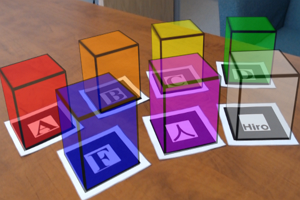
\includegraphics[width=7cm]{img/tracking/kanjo-hiro-marker.png}
    \caption[Kanji und Hiro Marker haben einfache geometrische Formen, Texte oder Buchstaben zur Erkennung in der Szene.]{Kanji und Hiro Marker haben einfache geometrische Formen, Texte oder Buchstaben zur Erkennung in der Szene\protect\footnotemark.}
    \label{fig: tracking_kanji_hiro}
\end{figure}

\footnotetext{https://stemkoski.github.io/AR-Examples/, zuletzt aufgerufen am 29.07.2022}

Die zweite Möglichkeit erfasst über Algorithmen der Computer Vision Merkmale in der realen Umgebung. Diese Art wird als \textit{marker-less AR} bezeichnet. Natürliche Merkmale können geometribasiert sein, indem Kanten oder Formen wie Vierecke erkannt werden. Bekannte Detektoren wie sind z.B. \textit{\acrfull{sift}}\cite{lowe1999} oder \textit{\acrfull{surf}}\cite{bay2008}. 

Diese Detektoren arbeiten nach einem ähnlichen Schema. Zunächst werden nach \textit{Schlüsselpunkten (engl. Key Points, Feature Points)} in einem Bild gesucht, die charakteristische Eigenschaften wie Punkte, Kanten, Kontrast oder homogene Regionen aufweisen.  Je nachdem wie groß das Bild ist und wie stark die Schwellwerte beim jeweiligen Detektor eingestellt sind, verändert sich die Anzahl an Schlüsselpunkten. Dies beeinflusst die Tracking Performance und die Genauigkeit. 
Ist eine finale Auswahl der Schlüsselpunkte erfolgt, erhält jeder Punkt einen sogenannten \textit{Deskriptor}. Dieser enthält lokale Eigenschaften auf dem Bild in der Umgebung des Punktes. Ziel eines Deskriptors ist es Schlüsslepunkte mit so wenig Informationen wie möglich eindeutig zu beschreiben. 
Sind die Deskriptoren vorhanden, kann im Anschluss ein \textit{Feature-Matching} durchgeführt werden. Dabei werden Schlüsselpunkte und Deskriptoren aus einer Datenbank\footnote{Dies kann ein vorgefertigtes Set an Schlüsselpunkten sein, die beispielsweise aus vorherigen Durchläufen entstanden sind. Meist enthält dies auch Informationen zu den Dimensionen des Objekts. Diese Datenbank wird \textit{Feature Map} genannt} mit den determinierten Deskriptoren verglichen und zugeordnet. Mithilfe der zugeorndeten Schlüsselpunkten kann die Pose der Kamera berechnet werden \cite[][]{doerner}\cite{herling2011}. Eine ausführliche Beschreibung der Algorithmen zu marker-less AR bietet Herling und Broll\cite{herling2011}.

\subsubsection*{Herausforderungen für marker-less Tracking in AR Anwendungen}

Damit eine valide Positions und Rotation berechnet werden kann, definieren Herling und Broll\cite{herling2011} Voraussetzungen für Detektoren. Da AR in Echtzeit abläuft, muss die Bestimmung von Schlüsselpunkten und Deskriptoren schnell berechnet werden. Weiterhin muss der Algorithmuss robust gegnüber unterschiedlichen Lichtverhältnissen sein. Dies gilt insbesondere bei AR in freier Umgebung, da sich die Lichtverhältnisse schnell verändern können. Da der Nutzer keine Einschränkungen in der Position der Kamera besitzt, kann ein schneller Perspektivwechsel erfolgen. Der Algorithmus muss daher eine Robustheit genüber starken Bildveränderungen haben. Letzlich muss eine Skalierungs-Invarianz bereitgestellt werden. Das bedeutet, dass das Tracking nicht auf eine bestimmte Entfernung beschränkt ist und weiter entfernte Punkte nicht verschwinden. In einem kleineren Bereich ist es einfacher Schlüsselpunkte zu detektieren. Die Skaleninvarianz ist daher insbesondere bei AR im Freien relevant.


Das \acrshort{sift} Verfahren Auch die aus der Robotertechnik bekannte \textit{\acrlong{slam}}\cite{slam1} \cite{slam2} Methode wird genutzt. 

\subsubsection{SIFT - Scale Invariant Feature Transform}
Vorteil dieser Methode ist, dass gleichzeitig eine 3D-Karte des Raumes generiert wird, die immer wieder zur Positions- und Rotationsbestimmung verwendet werden kann.

\subsubsection*{SURF}

\subsubsection*{SLAM}
Dabei werden entweder kamerabasiert (Visual SLAM) nach Merkmalen gesucht oder es kommen Sensoren zur Generierung von Tiefeninformationen zum Einsatz, z.B. Kinect \footnote{https://developer.microsoft.com/de-de/windows/kinect/} oder \textit{LIDAR-Sensoren (engl. light detection and ranging)}\cite{Liu2020}.

\subsubsection{GPS Tracking}
\label{tracking-gps-tracking}
Im Außenbereich wird bei AR auch GPS für das Tracking herangezogen. Dabei sind Positionsabweichungen von bis zu 10 Metern möglich, sodass eine genaue Bestimmung der extrinsischen Kameraparameter beeinträchtigt wird. Um die Tracking-Genauigkeit zu erhöhen, gibt es mehrere Methoden. \textit{DGPS (engl. Differential GPS)} verbessert GPS-Signale, indem es ein Korrektursignal durch eine ortsfeste Referenzstation mit bekannter Lokalisierung berechnet. Da es in Deutschland lediglich acht solcher Stationen gibt und einige Anbieter nur kommerziell die Daten bereitstellen, ist diese Methode nicht für diese Arbeit geeignet\footnote{https://www.heise.de/newsticker/meldung/Differential-GPS-und-WLAN-RTT-Praezise-Ortung-mit-Android-P-4046935.html} \footnote{Liste von DGPS-Sendern: https://www.ndblist.info/datamodes/worldDGPSdatabase.pdf}. Eine weitere bekannte Möglichkeit bietet \textit{SBAS (engl. Satellite Based Augmentation System)}, bei dem mehrere geostationäre Satelliten das GPS Signal auf bis zu einem Meter Genauigkeit zu verbessern \cite*{doerner}.

Platinsky und seine Koautoren\cite{platinsky} erstellen für ein besseres Tracking bei fehlender GPS Genauigkeit ein 3D-Modell der Umgebung. Bei der anschließenden AR Nutzung in diesem Gebiet wird auf dem Smartphone SLAM betrieben. Die Daten vom Smartphone werden mit der 3D-Karte verglichen, um ein genaueres Tracking durchzuführen. Ein ähnliches System wäre für die Anwendung in dieser Arbeit denkbar, da eine große Datenmenge von Bildern des Geländes vorhanden ist. Über Structure from Motion Methoden, kann mit den Bildern eine große 3D-Karte erstellt werden.